% Styles
\tikzset{
	smallBlock/.style = {rectangle, thick, minimum width=0.8cm, minimum height=0.8cm,text centered, draw=black, fill=white},
	midBlock/.style = {rectangle, thick, minimum width=2cm, minimum height=1.5cm,text centered, text width=3cm, draw=black, fill=white},
	bigBlock/.style = {rectangle, thick, minimum width=2cm, minimum height=2.5cm,text centered, text width=2cm, draw=black, fill=white},
	arrow/.style= {thick, black, ->, >=stealth},
	line/.style= {thick, black},
	textOutput/.style = {black,right},
	textInput/.style = {black,left},
	container/.style = {gray,dashed},
	sum/.style = {circle, minimum size=0.7cm, thick, draw=black, fill=white},
	%sum
	charge node/.style={inner sep=0pt},
	pics/sum block/.style n args={4}{
		code={
			\path node (n) [draw, circle, inner sep=0pt, minimum size=0.7cm] {}
			(n.north) +(0,-1.5mm) node [charge node] {$#1$}
			(n.south) +(0,1.5mm) node [charge node] {$#2$}
			(n.west) +(1.5mm,0) node [charge node] {$#3$}
			(n.east) +(-1.5mm,0) node [charge node] {$#4$}
			;
		}
	}
}
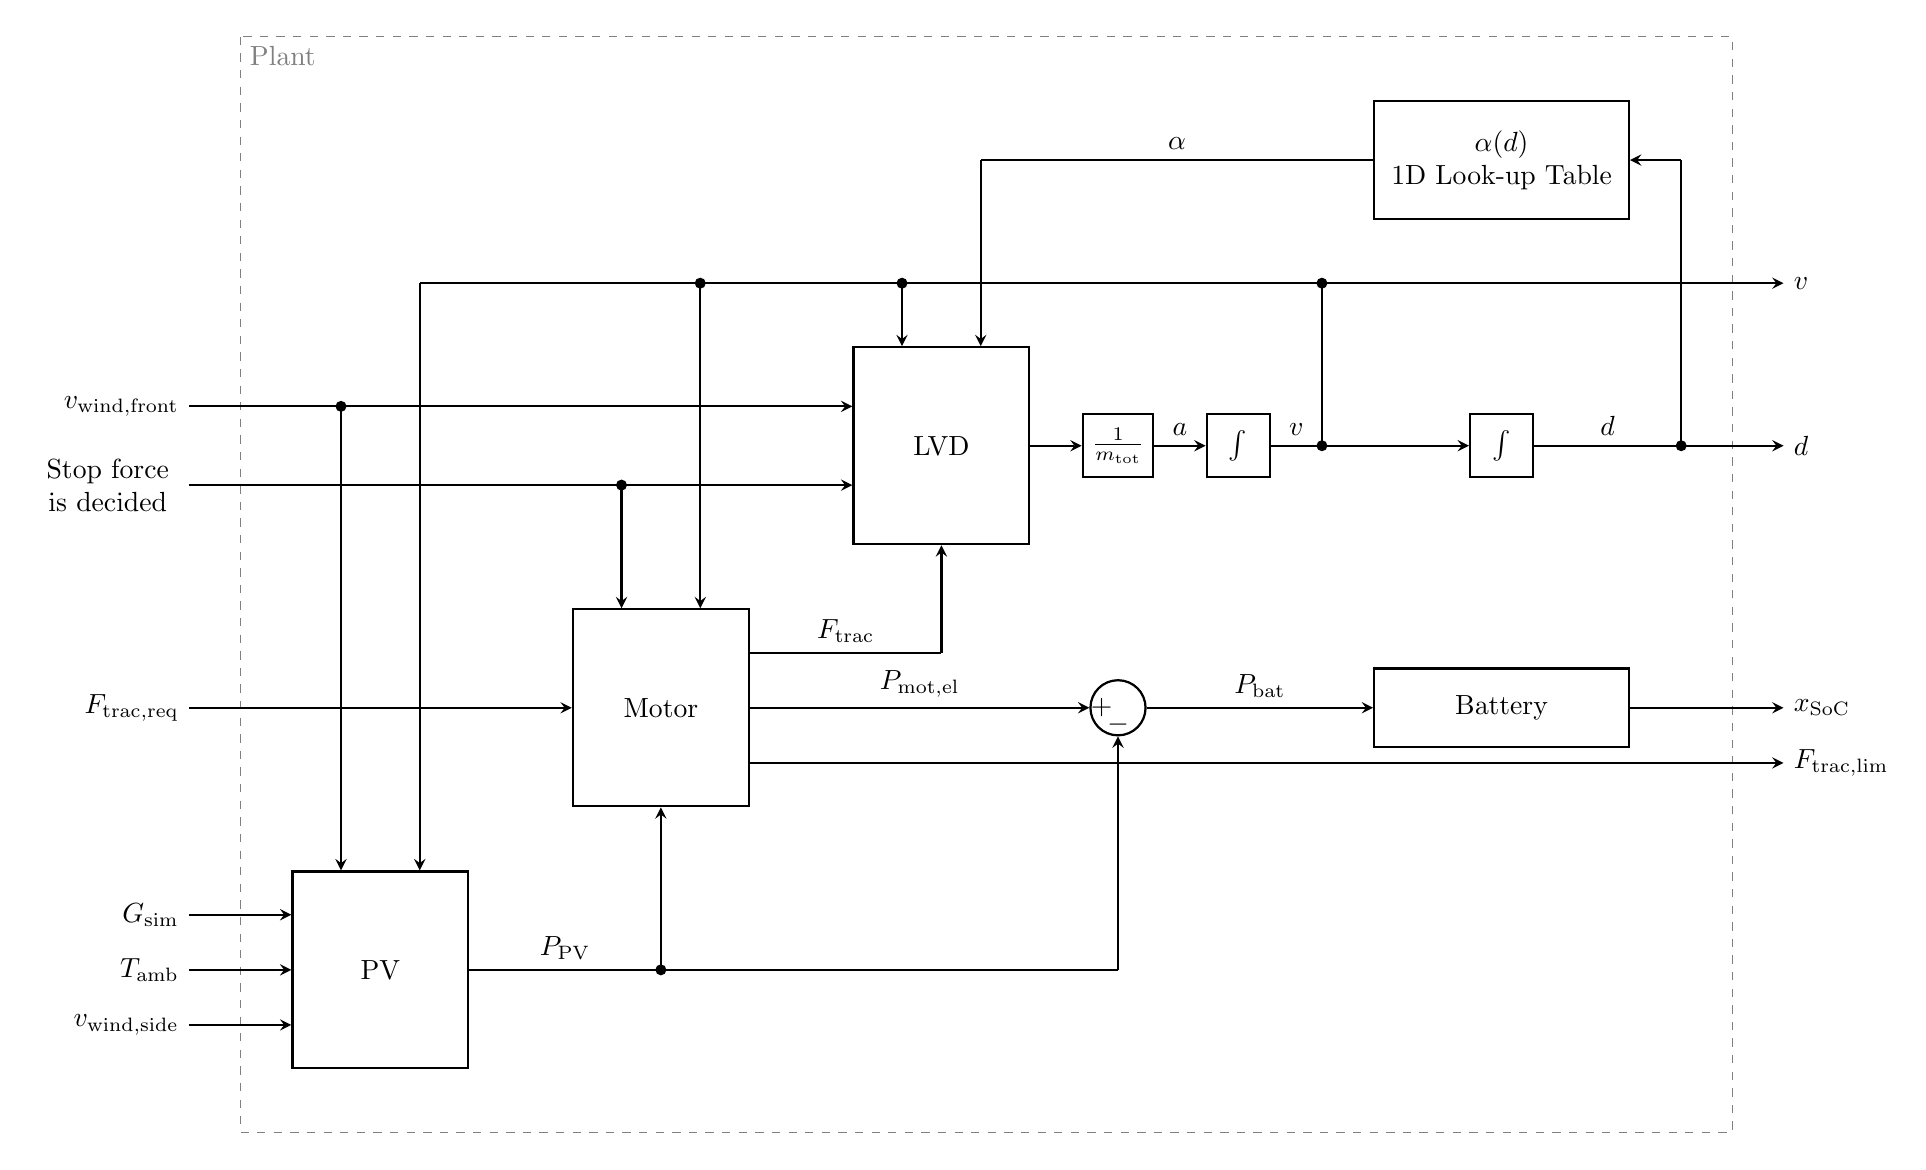
\begin{tikzpicture}
	% Definition
	%for three arrows
	\def\up{0.7}
	\def\down{-\up}
	\def\right{0.7}
	\def\left{-\right}
	%for two arrows
	\def\UP{0.5}
	\def\DOWN{-\UP}
	\def\RIGHT{0.5}
	\def\LEFT{-\RIGHT}
	%radius
	\def\radius{0.07}
	
	% Blocks
	\matrix[column sep=0.65cm, row sep=0.8cm]{
		%first row
		& \coordinate (c12); & & & &  & & & & &  & & & &
		\\
		%second row
		& & & & &  & \coordinate (c27); & & & &  \node[midBlock] (inclination) {$\alpha(d)$ \\ 1D Look-up Table}; & \coordinate (c212); & & &
		\\
		%third row
		& & \coordinate (c33); & & \coordinate (c35); &  & \coordinate (c37); & & & \coordinate (c310); &  & & & \coordinate (c314); &
		\\
		%fourth row
		\coordinate (c41); & & \coordinate (c43); & & \coordinate (c45); &  & \node[bigBlock] (lvd) {LVD}; & \node[smallBlock] (mass) {$\frac{1}{m_\mathrm{tot}}$}; & \node[smallBlock] (intAcc) {$\int$}; & \coordinate (c410); &  \node[smallBlock] (intVel) {$\int$}; & \coordinate (c412); & & \coordinate (c414); &
		\\
		%fifth row
		\coordinate (c51); & & & & \node[bigBlock] (motor) {Motor}; &  & \coordinate (c57); & \node[sum] (sum) {}; & & &  \node[midBlock, minimum height=1cm] (battery) {Battery}; & & & \coordinate (c514); &
		\\
		%sixth row
		\coordinate (c61); & & \node[bigBlock] (PV) {PV}; & & \coordinate (c65); &  & & \coordinate (c68); & & &  & & & &
		\\
		%seventh row
		& & & & &  & & & & &  & & \coordinate (c713); & &
		\\
	};
	
	% Container
	\draw[container] (c12) rectangle (c713);
	\node[gray, anchor=north west] at (c12.north west) {Plant};
	
	% Arrows;
	%to second row
	\draw[arrow] (c212) -- (inclination);
	\draw[line] (c412) -- (c212);
	\draw[line] (inclination) -- ([xshift=\RIGHT cm]c27) node[midway, above] {$\alpha$};
	%to third row
	\draw[arrow] ([xshift=\RIGHT cm]c33) -- (c314) node[textOutput] {$v$};
	\draw[line] (c410) -- (c310);
	\draw[arrow] ([xshift=\RIGHT cm]c27) -- ([xshift=\RIGHT cm]lvd.north);
	%to fourth row
	\draw[arrow] (c412) -- (c414) node[textOutput] {$d$};
	\draw[line] (intVel) -- (c412) node[midway, above] {$d$};
	\draw[arrow] ([yshift=\DOWN cm]c41) node[textInput, text width=1.8cm, text centered] {Stop force is decided} -- ([yshift=\DOWN cm]lvd.west);
	\draw[arrow] ([yshift=\UP cm]c41) node[textInput] {$v_\mathrm{wind,front}$} -- ([yshift=\UP cm]lvd.west);
	\draw[arrow] ([xshift=\LEFT cm]c37) -- ([xshift=\LEFT cm]lvd.north);
	\draw[arrow] (lvd) -- (mass);
	\draw[arrow] (mass) -- (intAcc) node[midway, above] {$a$};
	\draw[line] (intAcc) -- (c410) node[midway, above] {$v$};
	\draw[arrow] (c410) -- (intVel);
	\draw[arrow] ([yshift=\up cm]c57) -- (lvd);
	%to fifth row
	\draw[arrow] (battery) -- (c514) node[textOutput] {$x_\mathrm{SoC}$};
	\draw[arrow] (motor) -- (sum) node[midway, above] {$P_\mathrm{mot,el}$};
	\draw[arrow] (sum) -- (battery) node[midway, above] {$P_\mathrm{bat}$};
	\draw[arrow] ([xshift=\RIGHT cm]c35) -- ([xshift=\RIGHT cm]motor.north);
	\draw[arrow] (c68) -- (sum);
	\draw[line] (PV) -- (c65) node[midway, above] {$P_\mathrm{PV}$};
	\draw[arrow] (c65) -- (motor);
	\draw[arrow] (c51) node[textInput] {$F_\mathrm{trac,req}$} -- (motor.west);
	\draw[arrow] ([xshift=\LEFT cm, yshift=\DOWN cm]c45) -- ([xshift=\LEFT cm]motor.north);
	\draw[arrow] ([yshift=\down cm]motor.east) -- ([yshift=\down cm]c514) node[textOutput] {$F_\mathrm{trac,lim}$};
	\draw[line] ([yshift=\up cm]motor.east) -- ([yshift=\up cm]c57) node[midway, above] {$F_\mathrm{trac}$};
	%to sixth row
	\draw[arrow] (c61) node[textInput] {$T_\mathrm{amb}$} -- (PV);
	\draw[arrow] ([xshift=\RIGHT cm]c33) -- ([xshift=\RIGHT cm]PV.north);
	\draw[line] (PV) -- (c68);
	\draw[arrow] ([yshift=\up cm]c61) node[textInput] {$G_\mathrm{sim}$} -- ([yshift=\up cm]PV.west);
	\draw[arrow] ([yshift=\down cm]c61) node[textInput] {$v_\mathrm{wind,side}$} -- ([yshift=\down cm]PV.west);
	\draw[arrow] ([yshift=\UP cm, xshift=\LEFT cm]c43) -- ([xshift=\LEFT cm]PV.north);
	
	% Dots
	\fill [black] (c310) circle (\radius cm);
	\fill [black] ([xshift=\RIGHT cm]c35) circle (\radius cm);
	\fill [black] ([xshift=\LEFT cm]c37) circle (\radius cm);
	
	\fill [black] (c410) circle (\radius cm);
	\fill [black] (c412) circle (\radius cm);
	\fill [black] ([xshift=\LEFT cm, yshift=\DOWN cm]c45) circle (\radius cm);
	\fill [black] ([xshift=\LEFT cm, yshift=\UP cm]c43) circle (\radius cm);
	
	\fill [black] (c65) circle (\radius cm);
	
	%sum
	\path pic at (sum) {sum block={}{-}{+}{}};
	
\end{tikzpicture}